\documentclass{report}
\usepackage[utf8]{inputenc}
\usepackage{minted}
\usepackage[margin=0.7in]{geometry}

\usepackage{biblatex} %Imports biblatex package
\usepackage[toc,page]{appendix}
\usepackage{siunitx}
\usepackage{mathrsfs,mismath,amsfonts,amssymb,amsmath,mathabx, braket,diagbox,hhline,mathtools}
\usepackage{graphicx}
\usepackage{epstopdf}

\addbibresource{library.bib} %Import the bibliography file
\title{Continuous Error Correction in Quantum Dot Qubits}
\author{Stasiu Wolanski, Jesus College}
\date{2022 - 2023}

\begin{document}

\maketitle

\begin{abstract}
    Woop!
\end{abstract}

\tableofcontents

\section{Introduction}
\chapter{Background}

\section{Quantum error correction}
\subsection{Quantum computing}
\subsection{Error correction}
\subsection{Continuous error correction}


\section{Quantum Dot Qubits}
\subsection{Semiconductor Heterostructures}
\subsubsection{The Hubbard Model} \label{sec:hubbard_model}

\chapter{Theory}

\section{Rapidly repeated error correction schemes} \label{sec:repeat_analysis}
This section develops a framework for analysing error correction schemes that are based on discrete, but rapidly repeated, parity measurment and correction. It allows for the efficient and exact calculation of the expected fidelity of such a scheme given certain characteristic parameters: the rate of errors, the frequency of error correction cycles, and the fidelity of the error syndrome measurements.
The crucial insight is that all standard decoherence processes have the property that, when they are applied to a diagonal density matrix, the result is another diagonal density matrix. This means that by choosing a basis where the initial (codespace) state of the system is one of the basis vectors, we can analyse the system density matrix as a vector, and apply markovian evolution by calculating the relevant transition matrix.

\section{Truly continuous error correction in quantum dot systems} \label{sec:truly_continuous_theory}
\begin{figure}[h]
    \centering
    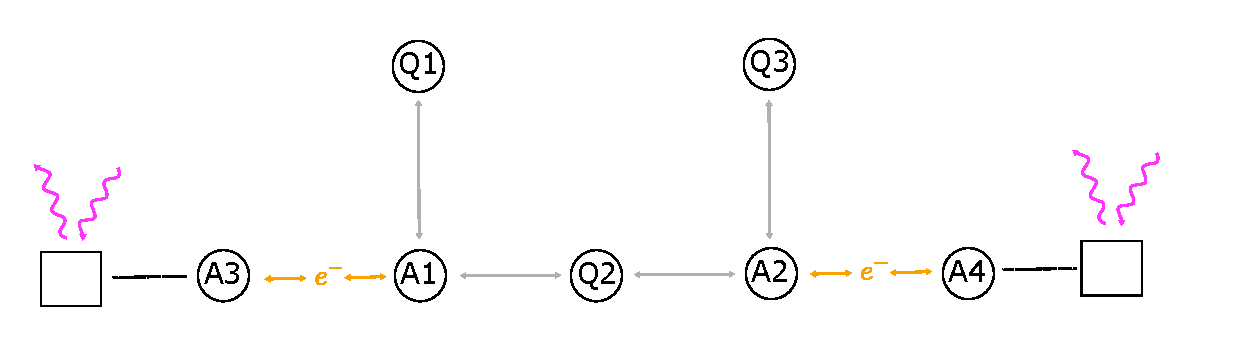
\includegraphics[scale = 0.9]{Figures/7q.pdf}
    \caption{Schematic of the layout of qubits for the continuous error correction scheme. Q1, Q2 and Q3 comprise a single logical qubit. A1 to A4 are ancilla qubits used to detect bit flip errors in the logical qubits. Q1 and Q2 are continuously weakly coupled to A1 through a tunnel barrier, and likewise Q2 and Q3 to A2. R1 and R2 are resonators, which are additional quantum dots held at a higher electron occupancy than the qubits. These are probed using RF signals, and their coupling to the charge on the ancillas then allows the singlet/triplet state of the ancillas, as in \cite{Oakes2022}.}
    \label{fig:7qubitlayout}
\end{figure}
\subsection{Scheme summary}

In this section a proposal for truly continuous error correction is developed. I thank Chris Long, Dr Mertig, Giovanni Oakes and my supervisor Dr Arvidsson-Shukur for contributing variously to the development of the ideas presented here. Recent developments in the field of RF reflectometry measurements enable the measurement of the singlet/triplet state of two adjacent qubits coupled via a tunnel barrier, by monitoring the rf reflection characteristics of a neighbouring electron reservior \cite{Oakes2022}. The codespace qubits are to be coupled pairwise to two ancilliary qubits whose function is to perform parity measurements, in such a way that any deviation from the codespace will result in a change of state of one or both of the ancilla qubits, depending on the error syndrome. The rate at which the error propogates to the ancilla qubit(s) is in the tens of nanoseconds, a faster timescale than either gate times (hundreds of nanoseconds) or readout (the state of the art \cite{Oakes2022} achives 6\unit{\micro\second}). 

This scheme is potentially more efficient than a repeated error correction scheme like those analysed in section \ref{sec:repeat_analysis}. One reason for this is that the `dead time' after an error has occurred during which the system is vulnerable to a second error is limited by the time for the ancilla to be reset, which is also on the order of microseconds (e.g. see \cite{Nakajima2019}). A second, more significant advantage is that the scheme does not require any quantum gates to be performed for the purposes of error sydrome detection, as such detection happens continuously and simultaneously with circuit gates. This reduces circuit complexity, and avoids the error accumulation associated with performing the syndrome measurements. 

TODO flesh this out.



The proposed qubit layout is given in figure \ref{fig:7qubitlayout}. The nature of the circuit requires a 2D array of quantum dot structures, of which there is not yet any published experimental demonstration, but a proposed architecture was proposed in \cite{Tadokoro2021_2}. In the scheme, the logical qubit is encoded in the \textit{odd parity subspace} of three qubits Q1, Q2, and Q3. There are two pairs of ancilla qubits: A1, A3, and A2, A4. Each of these is initially prepared in the $T_0$ triplet state. As shown in the figure, each pair of qubits Q1 and Q2, Q2 and Q3, is weakly coupled to one ancilla qubit through a voltage-controlled tunnel barrier. If the couplings are sufficiently well-tuned, the ancilla qubits will remain as triplets and no tunneling will occurr. When a bit-flip error occurrs on one of Q1, Q2 or Q3, this will cause one or both (depending on the error syndrome) of the ancilla pairs to rotate into a singlet state. This allows (subject to complexities discussed in section \ref{sec:tunneling_question}) tunneling between the electrons in the affected pair, which is registered as a change in dispersive response of the nearby resonator. Thus the error syndrome is immediately detected as a signal in the continuously monitored reflectometry circuit.

\subsection{Theoretical treatment of scheme with second order perturbation theory}

Suppose the system is initally in an arbitrary codespace state, with each of the ancilla pairs starting in triplet states:
\begin{equation*}
    \ket{\psi(t = 0)} = (\alpha\ket{\uparrow_{Q1}\downarrow_{Q2}\uparrow_{Q3}} + \beta\ket{\downarrow_{Q1}\uparrow_{Q2}\downarrow_{Q3}})(\ket{\uparrow_{A1}\downarrow_{A3}} + \ket{\downarrow_{A1}\uparrow_{A3}})(\ket{\uparrow_{A2}\downarrow_{A4}} + \ket{\downarrow_{A2}\uparrow_{A4}}) / 2
\end{equation*}
First consider the case where no coupling is applied between the qubits. If we can engineer our system so that $\delta_{1,3}^z = E_{A1}^z - E_{A3}^z \ll 1/T_1$, and similarly $\delta_{2,4}^z \ll 1/T_1$ (with $T_1$ the timescale of bit flip errors), then the energy difference between the two branches of each qubit singlet is sufficiently small that rate at which the triplets rotate into triplets, and so register a tunnelling event on the reflectometry apparatus, is long compared to the error time and so not limiting. We can see this by considering a single ancilla branch:
\begin{equation}
    \ket{\psi(t)} = \frac{1}{\sqrt{2}}(\ket{\uparrow\downarrow} + \exp(-2i\delta t)\ket{\downarrow\uparrow}) = \frac{1}{2}\ket{T_0}(1 + \exp(-2i\delta t)) + \frac{1}{2}\ket{S_0}(1 - \exp(-2i\delta t)))
\end{equation} \label{eq:triplet_to_singlet}, so that the amplitude of the singlet state goes as 
\begin{equation*}
    \left|\braket{S_0|\psi(t)}\right|^2 = \sin(\delta t)^2
\end{equation*}.

Now we apply a coupling between the following four pairs of qubits: Q1 and A1, Q2 and A1, Q2 and A2, Q3 and A2. We consider the four branches of the state in the computational basis of the ancilla qubits seperately, and apply second order perturbation theory to approximate the energy shift of each state due to the adiabatic application of a weak coupling, of strength $t$. The limits of this approximate treatment will be tested using a numerical simulation developed in chapter \ref{chap:methods}.

The standard formula for second order perturbation theory is (there is no first-order shift in energy as the perturbing terms are off-diagonal):

\begin{equation*}
    E_i^1 \approx E_i^0 + \sum_j{\frac{|\braket{\psi_i|V|\psi_j}|^2}{E_i^0 - E_j^0}}
\end{equation*} where $E_i^0$ and $E_i^1$ are the unperturbed and perturbed energies of state $i$, and $H_0$ and $V$ are the basic and perturbative hamiltonians. If we set $V$ to the hopping term in the hubbard model, then we obtain, for example,
\begin{align*}
    E_{\uparrow\downarrow\uparrow,\uparrow\downarrow,\uparrow\downarrow}^1 - E_{\uparrow\downarrow\uparrow,\uparrow\downarrow,\uparrow\downarrow}^0 &= 
    -\frac{t^2}{E_{\uparrow\updownarrow \uparrow,\varnothing\downarrow,\uparrow\downarrow}^0 - E_{\uparrow\downarrow\uparrow,\uparrow\downarrow,\uparrow\downarrow}^0}
    -\frac{t^2}{E_{\uparrow\varnothing \uparrow,\updownarrow\downarrow,\uparrow\downarrow}^0 - E_{\uparrow\downarrow\uparrow,\uparrow\downarrow,\uparrow\downarrow}^0}
    -\frac{t^2}{E_{\uparrow\updownarrow \uparrow,\uparrow\downarrow,\varnothing\downarrow}^0 - E_{\uparrow\downarrow\uparrow,\uparrow\downarrow,\uparrow\downarrow}^0}
    -\frac{t^2}{E_{\uparrow\varnothing \uparrow,\uparrow\downarrow,\updownarrow\downarrow}^0 - E_{\uparrow\downarrow\uparrow,\uparrow\downarrow,\uparrow\downarrow}^0}\\
    &= -t^2\left(\frac{1}{\Delta_1} + \frac{1}{\Delta_2} + \frac{1}{\Delta_3}+ \frac{1}{\Delta_4}\right)
\end{align*} with
\begin{align*}
    \Delta_1 &= U_{Q2} + \mu_{Q2} - \mu_{A1} + \E_{Q2}^z - \E_{A1}^z \\
    \Delta_2 &= U_{A1} + \mu_{A1} - \mu_{Q2} + \E_{Q2}^z - \E_{A1}^z \\
    \Delta_3 &= U_{Q2} + \mu_{Q2} - \mu_{A2} + \E_{Q2}^z - \E_{A2}^z \\
    \Delta_4 &= U_{A2} + \mu_{A2} - \mu_{Q2} + \E_{Q2}^z - \E_{A2}^z \\
\end{align*}, where the terms describe parameters of the Hubbard model described in section \ref{sec:hubbard_model}.

We note that $U_i \gg \Delta \mu_i, E^z_i$, and that the magnitude of $U_i$ (order of a few \unit{\milli\electronvolt}) varies little from site to site , so that we may define $\Lambda_t = 2t^2/\braket{U_i}$. Then we have 
\begin{equation*}
    E_{\mathrm{C}\uparrow\downarrow,\uparrow\downarrow}^1 - E_{\mathrm{C}\uparrow\downarrow,\uparrow\downarrow}^0  = \Delta E_{\mathrm{C}\uparrow\downarrow,\uparrow\downarrow} \approx
    \Delta E_{\mathrm{C}\uparrow\downarrow,\downarrow\uparrow} \approx
    \Delta E_{\mathrm{C}\downarrow\uparrow,\uparrow\downarrow} \approx
    \Delta E_{\mathrm{C}\downarrow\uparrow,\downarrow\uparrow} \approx -2\Lambda_t
\end{equation*}, where we note the shift in energy is the same, within the above approximations, for both of the codespace branches, $\ket{\uparrow\downarrow\uparrow}$ and $\ket{\downarrow\uparrow\downarrow}$, and denote the energies of both branches by the subscript C. All branches of the ancilla state will therefore accure phase at the same rate as long as the state code qubits remains within the codespace.

\newcommand{\dlam}[2]{\diagbox{$#1\Lambda_t$}{$#2\Lambda_t$}}
\begin{table}
    \centering
\begin{tabular}{|c|c||c|c|c|c|}
\hline
\multicolumn{2}{|c||}{Computational branch} & \multicolumn{4}{c|}{Ancilla branch} \\
\hline
 Subspace & branch & $\uparrow\downarrow\uparrow\downarrow$ & $\uparrow\downarrow\downarrow\uparrow$ & $\downarrow\uparrow\uparrow\downarrow$ & $\downarrow\uparrow\downarrow\uparrow$ \\
 \hhline{|=|=||=|=|=|=|}

Codespace & \diagbox{$\uparrow\downarrow\uparrow$}{$\downarrow\uparrow\downarrow$} & $2\Lambda_t$ & $2\Lambda_t$ & $2\Lambda_t$ & $2\Lambda_t$\\
\hline
E1 & \diagbox{$\downarrow\downarrow\uparrow$}{$\uparrow\uparrow\downarrow$} & \dlam{3}{1} & \dlam{3}{1} & \dlam{1}{3} & \dlam{1}{3}\\
\hline
E2 &\diagbox{$\uparrow\uparrow\uparrow$}{$\downarrow\downarrow\downarrow$} & \diagbox{$0$}{$4\Lambda_t$} & $2\Lambda_t$ & $2\Lambda_t$ & \diagbox{$4\Lambda_t$}{$0$}\\
\hline
E3 & \diagbox{$\uparrow\downarrow\downarrow$}{$\downarrow\uparrow\uparrow$} & \dlam{3}{1} & \dlam{1}{3} & \dlam{3}{1} & \dlam{1}{3}\\
\hline
\end{tabular}
\caption{Table of the (negative) energy shifts due to coupling of each ancilla branch, of each computational branch, of each subspace.}\label{table:shifts}
\end{table}


When a bit-flip error occurs, the state will aquire a component in one of the error subspaces, denoted E1, E2 and E3 depending on which qubit has flipped. Applying the above analysis, we calculate the energy shifts of each of the ancilla branches of each computational branch in each codespace. These are given in table \ref{table:shifts}. These shifts result in the A1, A3, or A2, A4 ancilla pairs rotating from triplets to singlets, or both, depending on the error subspace. To see this, consider the E1 error subspace, into which the state moves when the Q1 qubit experiences a bit-flip error. If both ancilla pairs are in triplet states at the point when the system transitions into the E1 subspace from the codespace, the state undergoes the following evolution \footnote{We assume that the resultant state is approximately a stationary state of the perturbed hamiltonian.}:

\begin{align*}
    \ket{\psi(t)} = &\alpha\ket{\downarrow\downarrow\uparrow}(
        e^{-3 i \Lambda_t t }\ket{\uparrow\downarrow\uparrow\downarrow} 
    + e^{-3 i \Lambda_t t }\ket{\uparrow\downarrow\downarrow\uparrow}
    + e^{-i \Lambda_t t }\ket{\downarrow\uparrow\uparrow\downarrow}
    + e^{-i \Lambda_t t }\ket{\downarrow\uparrow\downarrow\uparrow})/2 \\
    + e^{-i\delta_{Q1,Q3} t} &\beta\ket{\uparrow\uparrow\downarrow}(
        e^{- i \Lambda_t t }\ket{\uparrow\downarrow\uparrow\downarrow} 
    + e^{- i \Lambda_t t }\ket{\uparrow\downarrow\downarrow\uparrow}
    + e^{-3i \Lambda_t t }\ket{\downarrow\uparrow\uparrow\downarrow}
    + e^{-3i \Lambda_t t }\ket{\downarrow\uparrow\downarrow\uparrow})/2 \\
    &\approx e^{-3 i \Lambda_t t}\alpha\ket{\downarrow\downarrow\uparrow}
    (\ket{\uparrow\downarrow} + e^{2 i \Lambda_t t }\ket{\downarrow\uparrow})
    (\ket{\uparrow\downarrow} + \ket{\downarrow\uparrow})/2 \\
    &+ e^{- i \Lambda_t t}\beta\ket{\uparrow\uparrow\downarrow}
    (\ket{\uparrow\downarrow} + e^{-2 i \Lambda_t t }\ket{\downarrow\uparrow})
    (\ket{\uparrow\downarrow} + \ket{\downarrow\uparrow})/2
\end{align*}, where the $\delta_{Q1, Q3}$ phase term accounts for the difference in energy between the two branches, which is small compared to $\Lambda_t$, and irrelevant to our conclusion, so we ignore it. By comparison with equation \ref{eq:triplet_to_singlet}, we see that the A1,A3 ancilla pair in both branches will rotate into a triplet state with a characteristic timescale $1/\Lambda_t$. The same analysis yields for E2 error subspace:
\begin{align*}
    \ket{\psi(t)} \approx &\alpha\ket{\downarrow\downarrow\uparrow}
    (\ket{\uparrow\downarrow} + e^{ -2 i \Lambda_t t }\ket{\downarrow\uparrow})
    (\ket{\uparrow\downarrow} + e^{ -2 i \Lambda_t t }\ket{\downarrow\uparrow})/2 \\
    + e^{-4 i \Lambda_t t} &\beta\ket{\downarrow\downarrow\uparrow}
    (\ket{\uparrow\downarrow} + e^{ 2 i \Lambda_t t }\ket{\downarrow\uparrow})
    (\ket{\uparrow\downarrow} + e^{ 2 i \Lambda_t t }\ket{\downarrow\uparrow})/2
\end{align*}, so that both pairs of ancillas rotate into singlets. The E3 case is identical to the E1 case with the appropriate qubits exchanged, and leads to only the A2, A4 qubit pair rotating into a singlet.

\subsection{Further questions related to tunnelling physics} \label{sec:tunneling_question}

Much work has been done optimising the implementation and and examining the classical physics of reflectometry as a tool for quantum measurement. For a review see, e.g. \cite{Vigneau2023}, especially section VIII. During the project the author has not had time to study the physics behind this technique in detail. It appears, however, that present analyses treat the system semi-classically in assuming that an electron tunnels, or does not, within the measurement period (i.e. the period of time that the tunneling barrier between the pair of qubits is lowered). They then seek to maximise the fidelity with which this charge-shifting event, or lack thereof, is detected. This tunneling event is interpreted as a projective measurement of the singlet/triplet system at the point of measurement, with probabilities of either state given by Born's rule. In the present case this is an insufficient analysis: at any given time, there is necessarily some finite component of the electron pair state that is a singlet, and we need to establish a rate at which tunnelling occurs as a function of the amplitude of this component. A full treatment of this problem probably needs to be formulated in terms of quantum master equations and the theory of quantum decoherence \cite{Wiseman1996}.

Time has not permitted me to look into this issue, so at the suggestion of my supervisor I will make the simplifying assumption that any ancilla pair that aquires more than a 10\% square-amplitude of singlet immediately tunnels and is hence registered by the dispersive readout device with empirically determined fidelity.

\chapter{Methods} \label{chap:methods}

\section{Simulating the hubbard model}
This section will discuss the methodology used to perform simulations of scheme described in section \ref{sec:truly_continuous_theory} on a hubbard model of a multiple quantum dot system. The treatment of the error correction scheme described in section \ref{sec:truly_continuous_theory} is necessarily highly approximate due to the complexity of the high-dimensional hilbert space involved (for 7 electrons on 7 sites, the occupation basis is of dimension 3432) and the large number of parameters of the Hubbard model, so makes multiple simplifying assumptions, chiefly the application of second-order perturbation theory and ignoring the site-to-site variance in certain model parameters. It is therefore valuable to simulate the Hubbard model numerically to test the validity of these assumptions in various parameter regimes.

My supervisor Dr. Arvidsson-Shukur have developed a code (yet unpublished), \texttt{DotHamiltoniser}, designed to generate Hubbard hamiltonians in an occupation basis given a set of physical parameters ($E_i^z, U_i$, etc.), as well as to perform low-dimensional time-evolution simulations. This was very helpful at the start of my project to visualise the energy levels of the system and their dependence on coupling, but was not designed for higher dimensional time evolution, and could not be used for this purpose due to performance limitations.

I therefore designed a Hamiltonian simulation code, inspired by the work of Dr Arvidsson-Shuker et al., with the ability to handle higher dimensional systems. The system has three main components: 
\begin{enumerate}
    \item A python extension, \texttt{FastHamiltoniser}, written in C, C++ and CUDA, which provides highly performant specialised sparse matrix operations for use in Hamiltonian time evolution;
    \item \texttt{Hamiltonian}, a python class that builds a Hubbard model Hamiltonian from physical parameters; and
    \item \texttt{Evolution}, a python class which takes as input a Hamiltonian and a set of continuous time instructions to produce a time evolution of a given starting statevector.
\end{enumerate}
\subsection{Python extension: \texttt{FastHamiltoniser}}
\begin{figure}[h]
    \centering
    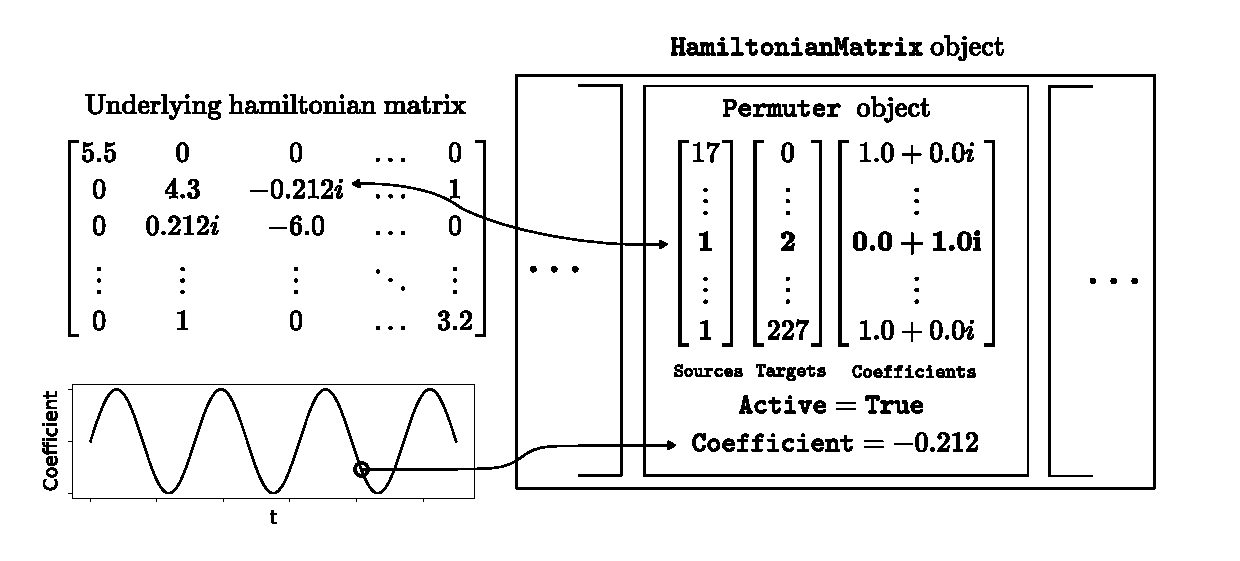
\includegraphics[scale = 0.8]{Figures/fasthamiltoniser/diagram.pdf}
    \caption{How sparse Hamiltonian matrices are represented in the custom python extension \texttt{FastHamiltoniser}. The non-zero matrix elements are grouped into objects of type \texttt{Permuter}, whose structure is calculated in advance but whose activation and multiplicative coefficients are modified efficiently as runtime.}
    \label{fig:fasthamiltoniser}
\end{figure}
\subsubsection{Structure of extension}
The purpose of the simulator is to solve the Schrödinger equation
\begin{equation} \label{eq:schrodinger}
    \dot{\psi} = -i H \psi 
\end{equation} (here expressed in natural units $\hbar = 1$) where $\psi$ is a vector in the occupation basis of a Hubbard Hamiltonian. In order to use Runge-Kutta \cite{Butcher1996} methods of integration, we need to be able to calculate this derivative efficiently at an arbitrary time and with arbitrary input. $H$ is typically very sparse, with the only off-diagonal terms given by magnetic drives and hopping couplngs, of which typically only a subset of size linear in the number of qubits are non-zero at a given time. 

To perform this calculation efficiently, I implemented the following data structure in C. A \texttt{HamiltonianMatrix} object, illustrated in figure \ref{fig:fasthamiltoniser}, contains basic data about the dimension of the array, as well as an array of pointers to objects of type \texttt{Permuter}. Each of these \texttt{Permuter} objects stores three arrays of equal length, two of integers representing source and target vector indices, and one of floats representing matrix coefficients, where each entry represents a matrix element. \texttt{Permuter}s also store a complex coefficient, which can be changed over time by writing to a single variable, and a boolean representing whether it is `on' or `off'. The internal arrays are determined in advance of the simulation by python code, and thereafter only the strength and activations of the \texttt{Permuter} objects need be modified during the simulation. For example, one such object provides all the on-diagonal elements of the matrix, and another might provide all the off-diagonal elements associated with a particular J-coupling between two qubits.

The calculation \ref{eq:schrodinger} can then be performed by iterating over the active permuters and building up the derivative vector according to the permutation and coefficient arrays. 
\subsubsection{Interaction picture calculation}
A further requirement that favoured the development of a custom C backend was the ability to perform simulations in the interaction picture. Performing simulations in the interaction picture is necessary due to the large differences in energy between eigenstates, for example due to the $U_i$ on-site repulsion in some states. With any choice of reference energy in a static basis, there are always states whose phase rotate much faster than the timescale of the evolutions that I wish to simulate, meaning there is no suitable step-size that captures the desired phenomena within reasonable computational time with the simulation remaining stable. Instead, we perform the following transformation to the interaction picture:
\begin{align*}
    \dot{\psi_i} &= -i\sum_j{H_{ij}\psi_j}\\
     \psi_i \rightarrow \phi_i &= e^{-i H_{ii} t} \psi_i \\
    \Rightarrow \dot{\phi} &= -i\sum_{j\ne i}{e^{- i (H_{jj} - H_{ii})t} H_{ij}\phi_j}
\end{align*}.

Since most off-diagonal terms $H_{ij}$ are zero at most points in time, this results in most states being stationary and lowering the rate of rotation of affected states to a longer timescale that can be simulated. It introduces the additional complexity, however, of introducing a time-dependence into the hamiltonian. I wrote a C function to perform the modified matrix multiplication, calculating the phase factors as required.

\subsubsection{GPU acceleration}
The calcluation to be performed is parallel in nature, and thus a candidate for GPU acceleration. I wrote the requisite kernels\footnote{This presented a lot of technical challenges as the process for incorporating CUDA C++ into python C extensions and compiling them is not documented and very technical. I made a template project with the setup to use in the future: https://github.com/Stasiu51/TemplateCudaEx} to perform the matrix multiplication in CUDA, a variant of C++ developed by Nvidia to control their graphics processing units (`GPU's) \cite{cuda}, one of which (a P620 Quadro) is installed in my laptop. On testing, the CUDA variant outperformed the CPU calculation only for systems with more than around 15 qubits, more than required and where the speed of computation is too slow for practical use anyway ($<10$ iterations per second, several orders of magnitude too slow for the simulations of the present project).

\subsection{Python class for Hubbard model construction: \texttt{Hamiltonian}}
This is a python class (and supporting code) that implements a Hubbard Hamiltonian, using \texttt{FastHamiltoniser} as a backend to store the underlying matrix. In particular it
\begin{enumerate}
    \item creates a list of basis vectors, represented as bit strings (with convenience functions for printing them in canonical notation), that span the fock basis of a system with a specified number of sites and number of electrons;
    \item defines creation and annhilation operators on these states, which it uses to
    \item construct the diagonal \texttt{Permuter} object that represents the self-energy terms due to chemical potential, coulomb repulsion, and static magnetic z-fields; and to
    \item construct the off diagonal \texttt{Permuter} objects generated by hopping terms and x and y magnetic fields. It also
    \item provides transformations to and from the interaction picture; and
    \item provides functions for creating projector and X matrices in the fock basis, which are more involved to calculate than in the computational (single electron per site) basis. 
\end{enumerate}

\subsection{Python class for time evolution of statevector: \texttt{Evolution}}

This class takes a reference to a \texttt{Hamiltonian} object, and a set\footnote{There is in fact only one such object, as they are defined in a recursive tree structure.} of objects that subclass the abstract base class \texttt{TimeStep} whose role is to provide instructions as to how to modify the parameters of the Hubbard model at given time. For example, one such object instructs the simulation to ramp a set of hopping couplings to a specified value over a given period of time, and another might oscillate the strength of the x component of the applied magnetic field at a given frequency and phase.

The \texttt{scipy} routine \texttt{solve\_ivp} is used along with the calculations of the derivative described above in a Runge-Kutta 5th order \cite{Butcher1996} integration routine to calculate the evolution of a given initial statevector. The routine is designed to estimate the errors and dynamically choose a step size for the integration. This works poorly in the present use case, as the calculated (vector-norm) error scales with the number of non-zero elements of the vector. Instead, the code allows the user to manually specify a step size, typically around $1/10$ of the smallest relevant timescale of the system, and checks the continued normalisation of the statevector as an imperfect check on the stability of the simulation.

Some demonstrations of the simulator and the results of a benchmarking exercise are shown in figure \ref{fig:benchmark}. 
\begin{figure}[h]
    \centering
    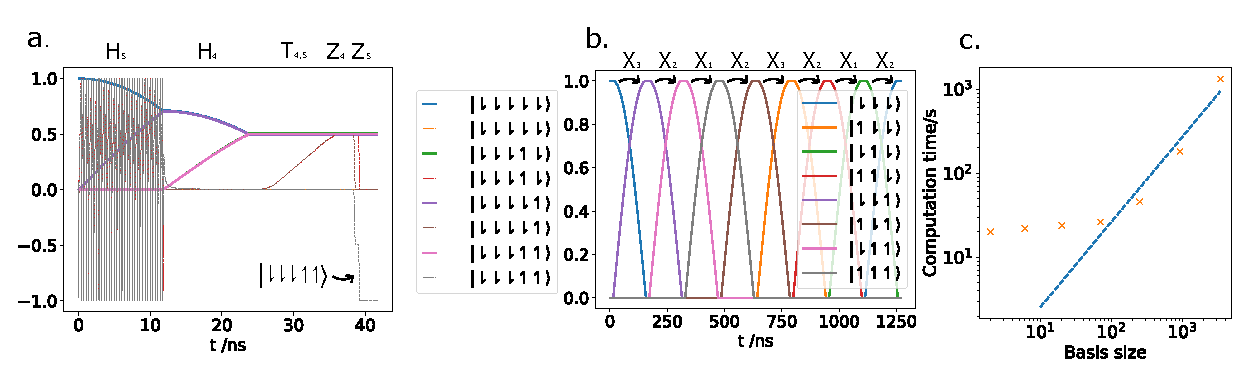
\includegraphics[scale = 0.85]{Figures/benchmark/benchmarks.pdf}
    \caption{Testing the capabilities of the simulation software. \textbf{a.} A plot of 5-qubit system showing the amplitudes (solid lines) and phases (dashed lines) of significant basis states. The plot demonstrates of a CPHASE gate acting on the last two qubits, so that the $\ket{\downarrow\downarrow\downarrow\uparrow\uparrow}$ state acquires a phase shift of $\pi$. First an X gate is applied to each of the two qubits, then a coupling between them is applied, and finally a z-rotation is applied by increasing the static field\protect\footnotemark. \textbf{b.} A sequence of X flips on a 3-qubit system. This circuit is generalised to N qubits to benchmark the simulator, with results given in \textbf{c.}. The results indicate a consistent speed of around 7.5 million statevector derivative elements calculated per second.}
    \label{fig:benchmark}
\end{figure}
\footnotetext{Applying a Z unitary rotation is not a capability typically built into such processors as it is unnecessary due to a technique called $Rz$ delaying (see, e.g. \cite{Nielsen2010} chapter 4.), but I implement it here to make the operation of the CPHASE clearer.}
\section{Truly continuous error correction prototype}
This section explains how the software described above was used to simulate the `truly continuous' error correction scheme developed in section \ref{sec:truly_continuous_theory}. In particular, we want to explore suitable physical parameters, such that when we initialise the system in an initial codespace state, and adiabatically turn on a weak coupling between the relevant qubits
\begin{itemize}
    \item the ancilla pairs remain in triplet states as long as the system remains in the codespace, for at least a time scale longer longer than ; and
    \item when a bit-flip error is artificially introduced, one or both of the ancilla pairs rotates into a singlet, as appropriate to the error syndrome.
\end{itemize}

\subsubsection{Physical parameters}
It is useful to survey the orders of magnitude of the various physical paramters of the experiment based on theoretical and experimental work to date. These can be found in table \ref{table:parameters}. As this is an exploratory piece of thoeretical work, I will take these as fairly liberal bounds.

\begin{table}
    \centering
\begin{tabular}{|c|c|c|c|}
    \hline
    Parameter & Symbol & Range & Example Reference\\
    \hline
    On-site coulomb repulsion & $U_i$ & $\sim 1\mathrm{Ry} \sim$ 1-10 \unit{\milli\electronvolt} & \cite{Shim2022}\\
    \hline 
    Static magnetic ($z$) field & $B_i^z$ & 1 - 10 \unit{\tesla} & \cite{Jock2018} \\
    \hline
    Variation in electron g factor & $\delta B_i^z$ &0.01 - 0.1 \unit{\mega\hertz} &\cite{Hwang2017} \\
    \hline
    Hopping coupling strength & $t_{ij}$ &$0.001 - 0.01$ \unit{\milli\electronvolt} & \cite{Veldhorst2015} \\
    \hline
    Phase flip coherence time &$ T_2^*$ & up to $10^3$\unit{\nano\second} in Si, $10^5$\unit{\nano\second} in $^{28}$Si & \cite{Loss2022}\\
    \hline
    Bit flip coherence/relaxation time &$T_1$&up to $10^6$\unit{\nano\second} in normal Si& \cite{Loss2022}\\
    \hline

\end{tabular}
\caption{Table of the (negative) energy shifts due to coupling of each ancilla branch, of each computational branch, of each subspace.}\label{table:parameters}
\end{table}

\subsection{Hubbard Hamiltonian setup} \label{sec:reduced_basis_approx}
The software enables us to set up a qubit basis that explicitly models the qubit layout shown in \ref{fig:7qubitlayout}, with three code qubits and two pairs of ancilla qubits. This seven-qubit system has a fock basis of dimension 3432, which is just about feasible to simulate using the software I developed (simulations of sufficiently small time step take several minutes each, and there are memory limitations in storing the results). However, this can be sped up by noting that in the circuit to be simulated, the second of each pair of ancillas, A3 and A4, do not experience any coupling, so the hamiltonian is always diagonal in these dimensions. Furthermore, the ancilla part of all states that are non-zero in the simulation are constructed out of the $\ket{\uparrow\downarrow}$ and $\ket{\downarrow\uparrow}$ states with respect to these pairs of qubits, as well as non-computational states. Therefore, we may reduce our basis if we make an appropriate modification to the Hamiltonian:
\begin{align*}
    \ket{\dots \uparrow\downarrow\uparrow\downarrow} &\rightarrow \ket{\dots \uparrow\uparrow} &
    \ket{\dots \uparrow\downarrow\downarrow\uparrow} &\rightarrow \ket{\dots \uparrow\downarrow}\\
    \ket{\dots \downarrow\uparrow\uparrow\downarrow} &\rightarrow \ket{\dots \downarrow\uparrow} &
    \ket{\dots \downarrow\uparrow\downarrow\uparrow} &\rightarrow \ket{\dots \downarrow\downarrow}\\
    E_{A1}^z &\rightarrow E_{A1}^z - E_{A3}^z & E_{A2}^z &\rightarrow E_{A2}^z - E_{A4}^z
\end{align*} this does not affect the energy levels of any of the computational states, and only affects the non-computational basis states by a quantity of order $E_i^z \ll U_i$. If we accept this approximation, we can reduce our basis size to 252, which increases the simulation speed by a factor of around $14 - 20\times$ (this is a non-linear speedup as all the simulation data now fits into memory).

Also note that most variation in spin energy from site to site come from variation in the electron G factor at different sites rather than inhomogenaities in the magnetic field \cite{Hwang2017}. It is convenient and equivalent, however, to simply include these variations into the magnetic field\footnote{Although my software does have the capability to vary the electron g-factor from site to site, it is simpler not to use it. }

\subsection{Energy shifts due to hopping coupling}

\begin{figure}[h]
    \centering
    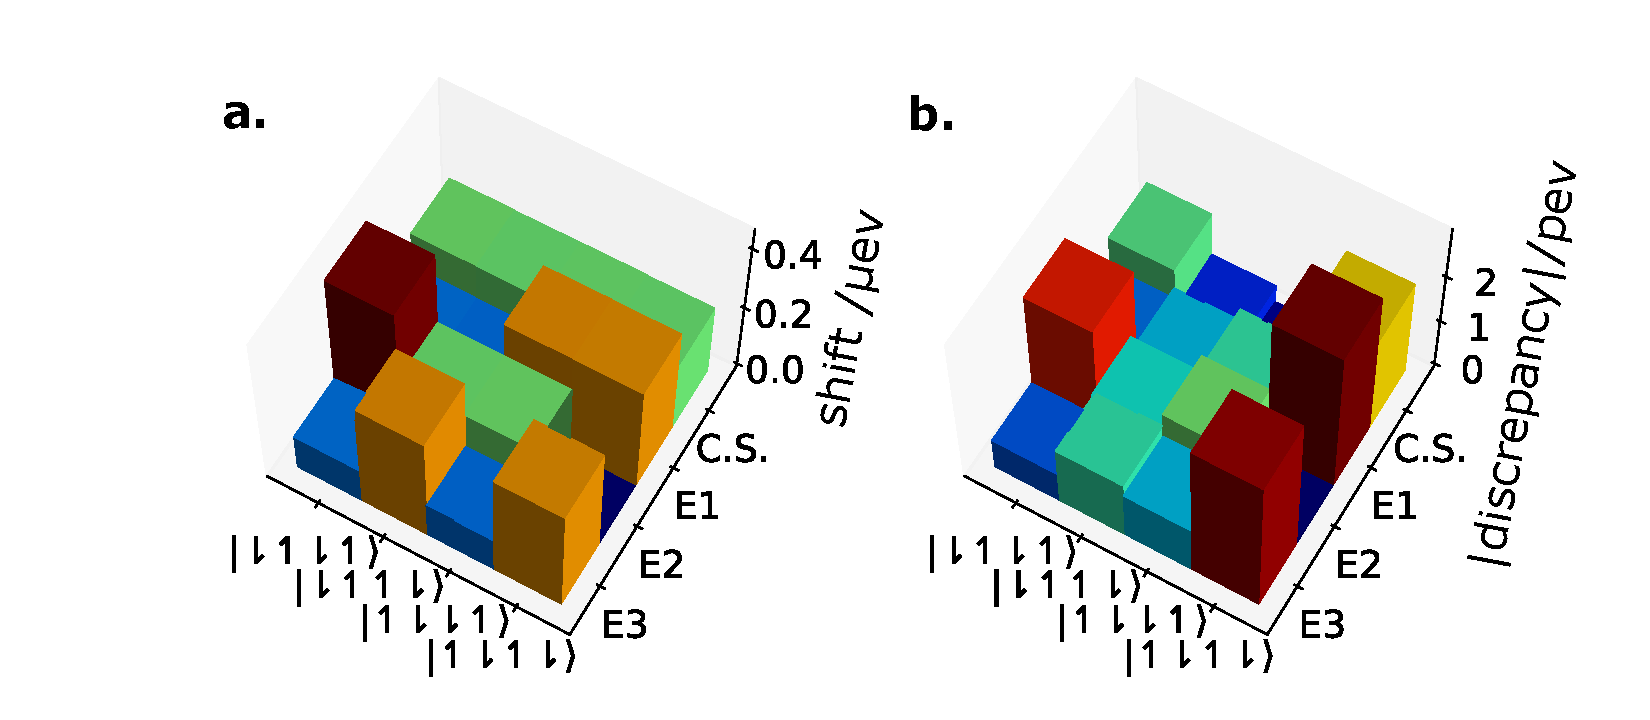
\includegraphics[scale = 0.4]{Figures/shifts.pdf}
    \caption{\textbf{a.} shows the calculation of energy shifts of the various relevant computational basis states calculated with a coupling of $0.015\unit{\milli\electronvolt}$ applied. Only one branch $\ket{\uparrow\downarrow\uparrow}$ of the computational state in each subspace is shown. This can be compared with the second order perturbation theory result calculated in table \ref{table:shifts}. The (absolute value of) the descrepancy between the simulation and the perturbation theory result is given in \textbf{b.}. Note the scale in the second plot.
    \label{fig:shifts}}
\end{figure}
It is important to know the energies of the perturbed computational states for two reasons: firstly, in order to validate the second-order perturbation theory results in section \ref{sec:truly_continuous_theory}; and secondly knowing the exact energies of these states is important if one is to use oscillating microwave signals to drive transitions between the states, to implement unitary rotations on the qubits while the coupling is active.

We find these by the following procedure: we initialise the system in the computational basis state of interest, and the hamiltonian with all couplings zero. we perform an interaction picture simulation where the couplings are ramped up to the steady state value over a time period that is sufficiently long so as to ensure adiabatic evolution of the state ($100\times\braket{U_i}^{-1}$ as this is the shortest timescale in the system). We compare this state to a list of the eigenvectors of the matrix generated by the Hamiltonian with the coupling at full strength. The eigenvector which has the maximal inner product with this state (the inner product is close to unity for the correct state, and close to zero otherwise) is the perturbed eigenvector associated with the original state in the computational basis state, and we take the associated eigenvalue as the perturbed energy.

The results for a coupling of 0.015\unit{\milli\electronvolt}, which is slightly higher than a typical coupling, and other typical experimental parameters, are given in figure \ref{fig:shifts}. The simulation agrees with the perturbation theory calculation within 1\%. The agreement is closer for smaller coupling values.

\subsection{Demonstrating the error propagation}
We now want to demonstrate the process of propagation by which bit-flip errors in the code qubits Q1, Q2, Q3 result in the relevant ancilla pairs rotating into singlets, or in the reduced basis approximation decribed in \ref{sec:reduced_basis_approx}, the qubits A1 and A2 rotating from $(\ket{\uparrow} + \ket{\downarrow})/\sqrt{2}$ to $(\ket{\uparrow} - \ket{\downarrow})/\sqrt{2}$, which is approximately equivalent.

We can acheive this by initialising the code qubits in the codespace, and then adiabatically turning on the coupling. We let this system run in steady state for enough time to establish the rate at which the singlets are introduced in the codespace. We then instantaneously apply an X unitary on one of the qubits by, and continue to let the simulation run. Afterwards, we can project the resulting time-evolved statevector data into the singlet and triplet spaces. The system prior to the bit flip is shown in figure \ref{fig:beforeflip}, and the behvaiour when a bitflip is introduced mid-way through the simulation is shown in figure \ref{fig:afterflip}.
\begin{figure}[h]
    \centering
    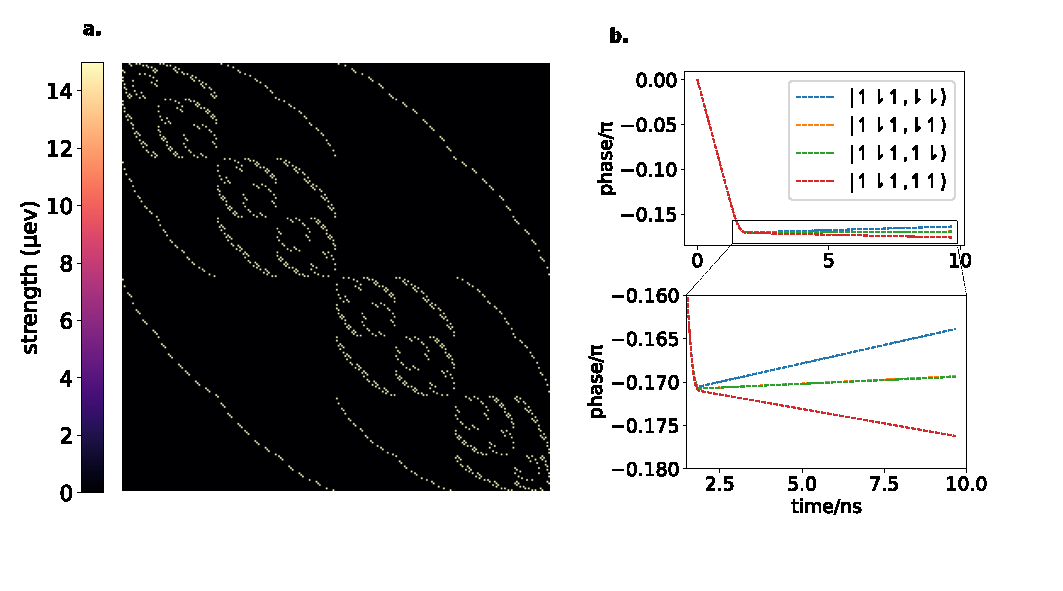
\includegraphics[scale = 1]{Figures/singlettriplet.pdf}
    \caption{The effect of applying the hopping coupling to the system still inhabilting the codespace. \textbf{a.} shows the (elementwise absolute value of the) hamiltonian matrix in the interaction picture at full strength. \textbf{b.} shows the rate of aquisition of phase of the relevant basis states. The phase initially drops when the coupling is applied, and then the states slowly drift apart from one another in phase due to the difference in electron g-factor of around 30 \unit{\mega\hertz}. At this rate, the triplet will `flip' into a singlet after around 200 \unit{\nano \second}, so this combination of parameters (coupling strength = 0.015 \unit{\milli\electronvolt}) is not be suitable for error correction. The inhomeneity between the sites needs to be reduced.
    }\label{fig:beforeflip}
\end{figure}

\begin{figure}[h]
    \centering
    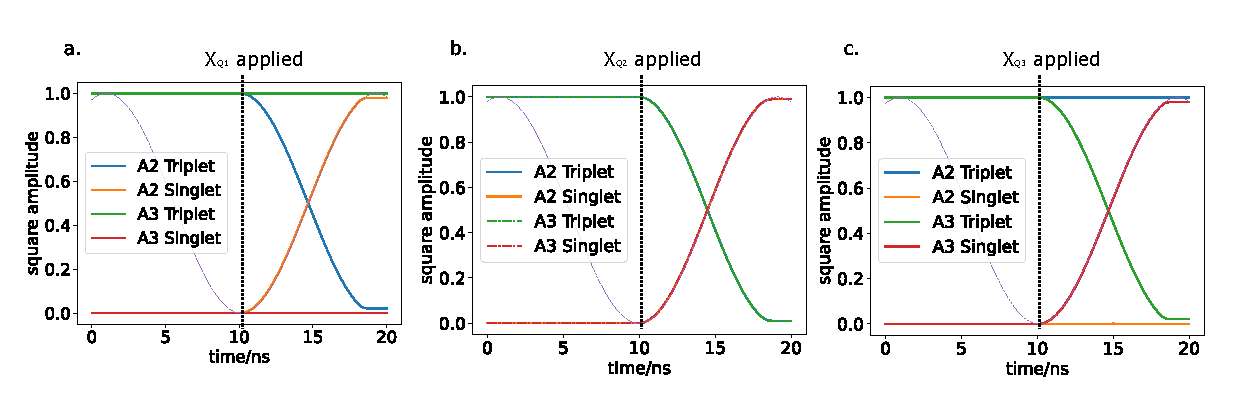
\includegraphics[scale = 0.87]{Figures/flips.pdf}
    \caption{Demonstrating the expected behaviour of the ancillas when a bit flip error is artificially introduced on one of the code qubits: Q1 is flipped in \textbf{a.}, resulting in a rotation of the A2 ancilla; Q2 is flipped in \textbf{b.}, resulting in \textit{both} A2 and A3 rotating, and Q3 is flipped in \textbf{c.}, so that A3 rotates only. In each case, the purple dashed line shows the expected frequency of rotation derived in section \ref{sec:truly_continuous_theory}, $\Lambda_t$. The dotted purple line shows the arbitrily set threshold for detection. Note that the period of rotation is much faster than the other typical timescales of quantum dot qubit systems.
    }\label{fig:afterflip}
\end{figure}


\chapter {Feasibility of the scheme}
There are features of this scheme which are potentially attractive, such as the fact that it does not require error correction steps to be programmed into a circuit, and the essentially instantaneous error detection that should lead to reduced `dead time'. However, the above proposal is unlikely to be practical as a means of increasing electron fidelity with current experimental parameters. 

The main problem with this scheme is that it only provides a way to protect against bit flip errors. The typical coherence time for such `relaxation' processes, $T_1$ in silicon systems is typically in the hundreds of microseconds or a few milliseconds \cite{Loss2021}\cite{Zwerver2022}; the best performance in this respect is isotopically purified $^{28}$Si, in which all atomic nuclei have zero spin. The more pressing limitation for such systems are phase-flip errors, whose coherence times $T_2^*$\footnote{$T_2^*$ is the `effective' decoherence time taking into account unknown but constant inhomogeneities in the system and applied field, whereas $T_2 > T_2^*$ is for decoherence cause by purely random environmental noise. $T_2^*$ is normally the more relevant quantity.} are typically 1-3 orders of magnitude shorter \cite{Loss2021}. I can see no obvious way to extend the scheme as described here to phase-flip errors. The issue is that most discrete error corrections can make use of the fact that phase- and bit- flip errors are equivalent up to a change of basis $\ket{0} \leftrightarrow \ket{+}$, $\ket{1}\leftrightarrow\ket{-}$, and just transform into the appropriate basis before the error correcting step using Hadamard gates. This is not possible in a continuous scheme like the one described here.

Even if we restrict ourselves to trying to reduce errors due to relaxation and leave phase-flip correction to other techniques, there are still limitations due to the inhomogeneities of silicon systems. In order for the correction to provide an improvement to the current $T_1$ times of order milliseconds, the time it takes the ancillas rotate into singlets whilst the system is in the codespace longer than this. This requires the overall spin difference $\delta_{A1, A3} = E_{A1}^z - E_{A3}^z$ and $\delta_{A2, A4}$ to be significantly less than $1/T_1 \approx 1\unit{\kilo\hertz}$, which is smaller than the expected range \cite{Hwang2017}.

During the course of the project I also developed a highly theoretical error-correction scheme that in principle could correct against both phase flip and bit flip errors. This I describe in appendix \ref{chap:lockedstates}. 
\section{Conclusions}

\printbibliography % TODO lots of incomplete references!

\begin{appendices}
\chapter{Decoherence theory}
Decoherence in qubits is commonly decomposed into two main channels: phase damping and amplitude damping. Amplitude damping is concerned with processes of relaxation that cause a qubit in the higher energy $\ket{1}$ state (in my project this is represented with a spin-up electron on a qubit) to the $\ket{0}$ state. Since these states have different energies, this process is asymmetrical: relaxation requires emission of a photon and occurs at a higher rate than the reverse process, electron promotion via absorption. 

The rate of amplitude damping, $T_1$ in silicon ranges from the order of milliseconds (e.g. 5\si{ms} in Giovanni's 2022 Paper) to seconds (20s in D. Keith et al 2019), which is between 4 and 7 orders of magnitude slower than typical gate operation times of hundreds of nanoseconds and 3-6 orders of magnitude than the best (RF reflectometry) readout times, which are 1.5\si{\micro s} in D Keith and 6\si{\micro s} in Giovanni's paper - note these give different fidelities and are just to give an idea of order of magnitude. These techniques, like the original Elzerman readout readout, rely on a spin-selective tunneling process with some known rate. Dephasing rates, $T_2$ and $T_2^{*}$, are much faster in silicon than $T_1$: the best recorded $T_2^*$ is (I think) 270\si{\micro s} in isotopically purified silicon (Tyryshkin et al. 2012). Since this is more comparable to the gate operation and crucially readout times, and it is a much greater problem, I will focus on trying to mitigate dephasing through a $\ket{+++}, \ket{---}$ three-bit code.


Amplitude damping has krauss operators (see, e.g. Nielsen and Chuang):
\begin{align*}
E_0 &= \begin{bmatrix}
1 & 0\\
0 & \sqrt{1-\gamma} 
\end{bmatrix}   &   E_1 &= \begin{bmatrix}
0 & \sqrt{\gamma}\\
0 & 0 
\end{bmatrix}\\
\end{align*}
where gamma can be thought of as the probability that a photon is lost in the time interval the krauss operators describe. These have the following effect on a density matrix:
\begin{equation*}
    \begin{bmatrix}
        \rho_{00} & \rho_{01} \\ \rho_{10} & \rho_{11}
    \end{bmatrix}
    \longrightarrow
    \begin{bmatrix}
        \rho_{00} + \gamma \rho_{11} & \sqrt{1-\gamma} \rho_{01} \\ \sqrt{1-\gamma} \rho_{10} & (1-\gamma) \rho_{11}
    \end{bmatrix}
\end{equation*}
The other decoherence channel of interest is phase damping. This is the channel we must worry about if we wish to preserve the fidelity of electrons in a $\ket{+} = (\ket{0} + \ket{1})/\sqrt{2}$ state, as its rate is generally much greater than that of amplitude damping in silicon. Intuitively, one imagines where stray and unknown EM fields shift the realtive energies of the $\ket{1}$ and $\ket{0}$ states, resulting in a phase drift of the qubits over time, which, for our ignorance of the specifics, we might model as Brownian motion:
\begin{equation*}
\alpha\ket{0} + \beta\ket{1} \longrightarrow \alpha\ket{0} + \exp(-i W(\Delta t) \sqrt{2\lambda}) \beta\ket{1}
\end{equation*}
where $W(\Delta t)$ is a Wiener process, that is, a Gaussian random variable with units of $t^{1/2}$ with $\mathbf{E}[W(\Delta t)] = 0$ and $\mathbf{Var}[W(\Delta t)] = \Delta t$. $\lambda$ is the rate of wander with units of inverse time. This process results in a transformation on a general density matrix:
\begin{equation} \label{eq:phasedamptrans}
    \begin{bmatrix}
        \rho_{00} & \rho_{01} \\ \rho_{10} & \rho_{11}
    \end{bmatrix}
    \longrightarrow
    \begin{bmatrix}
        \rho_{00} & e^{-\Delta t \lambda} \rho_{01} \\ e^{-\Delta t \lambda} \rho_{10} & \rho_{11}
    \end{bmatrix}
\end{equation} or using Krauss operators:
\begin{align*}
E_0 &= \begin{bmatrix}
1 & 0\\
0 & e^{-\Delta t \lambda}
\end{bmatrix}   &   E_1 &= \begin{bmatrix}
0 & 0\\
0 & \sqrt{1-e^{-2\Delta t \lambda}}
\end{bmatrix}\\
\end{align*}
This process, although apparently qualitatively different, is mathematically equivalent to a Poisson `phase-flip' process with rate $\lambda$, in which case we have
\begin{equation*}
\alpha\ket{0} + \beta\ket{1} \longrightarrow 
\begin{cases} 
      \alpha\ket{0} - \beta\ket{1} & p\\
      \alpha\ket{0} + \beta\ket{1} & 1-p \\
   \end{cases}
\end{equation*} where the probability of ending up flipped at the end of the time interval is
\begin{equation}\label{eq:p_def}
    p = e^{-\Delta t \lambda}\left(\frac{\lambda}{1!} + \frac{\lambda^3}{3!} \cdots\right) = \frac{1}{2}(1-e^{-\Delta t \lambda})
\end{equation}
it is then straightforward to verify this gives the same density matrix transformation as in (\ref{eq:phasedamptrans}). This equivalence gives an intuitive way of understanding the futility of attempting to preserve the state of the state undergoing Brownian phase motion through the quantum Zeno effect: measurement has no effect on states that are already an eigenstate of the measurement. Mathematically this is easiest to see by transforming to the $\ket{+}$, $\ket{-}$ basis, where a mixed state whose eigenstates are basis states transforms as follows:
\begin{align*}
    \begin{bmatrix}
        \rho_{++} & 0\\ 0 & \rho_{--}
    \end{bmatrix}
    \longrightarrow
    &\begin{bmatrix}
        \frac{1}{2}(1+e^{-\Delta t \lambda})\rho_{++} + \frac{1}{2}(1-e^{-\Delta t \lambda})\rho_{--} & 0 \\
        0 & \frac{1}{2}(1-e^{-\Delta t \lambda})\rho_{++} + \frac{1}{2}(1+e^{-\Delta t \lambda})\rho_{--}
    \end{bmatrix}\\
    = &\begin{bmatrix}
        (1-p)\rho_{++} + p\rho_{--} & 0 \\
        0 & p\rho_{++} + (1-p)\rho_{--}
    \end{bmatrix}\\
\end{align*}
In this basis we may write:
\begin{equation*}
    \rho \longrightarrow (1-p)\rho + p X\rho X
\end{equation*}
So after the decoherence has been applied, whatever the underlying process, we may consider the system to still be a purely probabilistic mixture of $\ket{+}$ and $\ket{-}$, decaying to the maximally mixed state as $\Delta t \rightarrow \infty$.

This result, which extends naturally to the $N$ qubit case, opens the door to a purely Markovian analysis of complex error correction schemes.

\subsubsection{Explanation in terms of Coherence Theory}
The theory of coherence quantification, set in motion by Baumgratz et al. in 2014 with their paper `Quantifying Coherence', seeks to treat quantify quantum coherence as a resource to be used up by decohering operations. The development of this theory has led to the definitions of \textit{incoherent} (from the original paper) and \textit{strictly incoherent} (Yadin et al 2016) quantum operations. The theory requires the definition of a fixed basis with respect to which coherence is measured (the $\ket{+}$ is only incoherent in the $\ket{+}$, $\ket{-}$ basis, for instance).

An incoherent operation is defined as one that maps incoherent states, states which are diagonal in the chosen basis, to other diagonal states. The definition given is that for an operation defined by Krauss operators $\{E_\mu\}$, for each of the $E_\mu$:
\begin{equation*}
    E_\mu \sum_i p_i \ket{i}\bra{i} E_\mu^\dag = \sum_i q_i \ket{i}\bra{i}
\end{equation*}
While not mentioned by the authors, it is straightforward to show that the property of incoherence of an operation, in contrast to the property of incoherence of a \textit{state}, is unitarily invariant, that is, an operation that is incoherent in one basis is necessarily incoherent in all others. In addition, it is obvious that an operation whose Krauss operators are chosen from the (possibly scaled) Krauss operators of other incoherent operators is itself incoherent. Within this framework it is easy to see why amplitude damping, bit flip (both manifestly incoherent in the computational basis), phase flip (manifestly incoherent in the $\ket{+}$, $\ket{-}$ basis), and phase-bit flip (manifestly incoherent in the $(\ket{0} \pm i\ket{1})/\sqrt{2}$ basis) channels as well as combinations of the above such as the depolarising channel are all incoherent operations. Of these, the amplitude damping and bit-flip channels are further \textit{strictly incoherent}, meaning the measurement statistics of the state after their application are independent of the off-diagonal elements of the state prior to the application. The theory of quantifying coherence then requires that any useful measure of coherence monotonically decrease under the application of these operations. In our case, we start in a incoherent state, so for all such measures $\mathcal{C}$, $\mathcal{C}(\rho_0) = 0$, which remains true for all subsequent time.

\chapter{Detecting errors in ancilla qubits.}
One problem the error correction scheme described in section \ref{sec:truly_continuous_theory} is that it is enturely vulnerable to errors ocurring in the ancilla qubits. If one such error did occur, the system would assume the resulting tunneling event was a result of a code qubit error and apply an erroneous correction gate, which would then push the system irreversibly out of the codespace.
\begin{figure}[h]
    \centering
    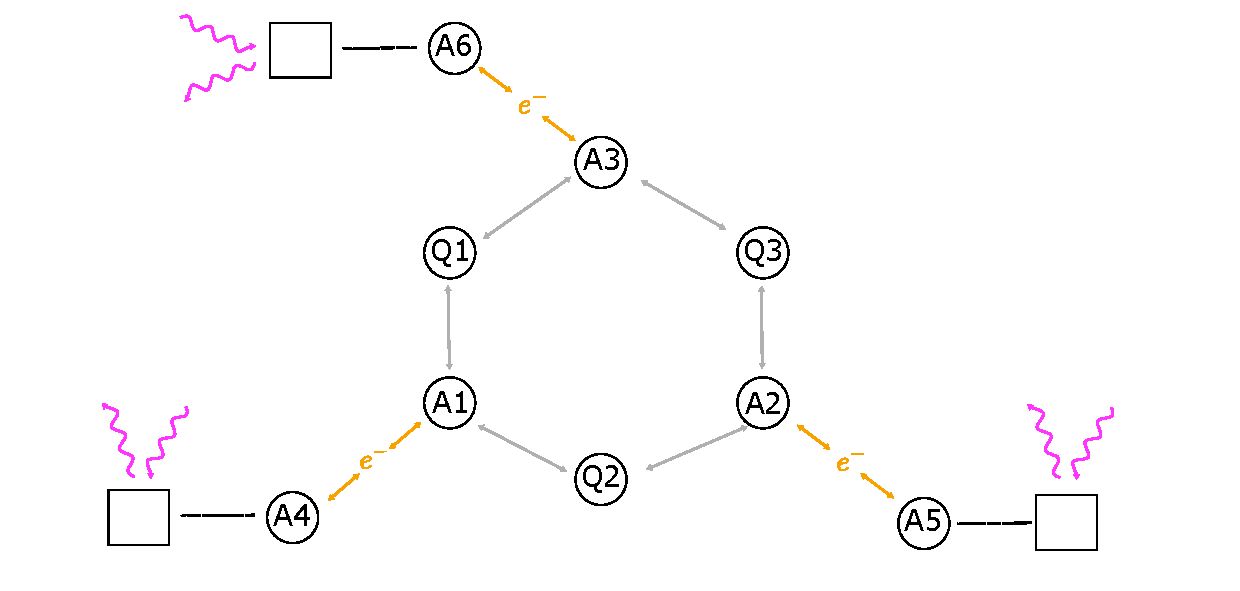
\includegraphics[scale = 0.9]{Figures/9q.pdf}
    \caption{The modified qubit layout that would allow for detection of ancilla errors.}
    \label{fig:9qubitlayout}
\end{figure}
Figure \ref{fig:9qubitlayout} shows a layout tht incorporates redundancy into the ancilla measurements. With this setup, the system would always expect to see two ancilla tunneling events in case of an error in the code qubits. If only one tunneling event was detected, the system could assume that the error was only in the that ancilla system, and reset it without taking the code qubits out of the codespace.

The limitation in implementing a scheme such as this one is at present topological; there has not yet been any experimental demonstration of 2D qubits arrays large enough for such a system.
\chapter{Locked states}
The purpose of this section a system that is continuously sensitive to both phase- and bit-flip errors. I will describe a set of what I call `locked states' which have the property that either a spin or phase flip results in an immediately visible charge movement, and suggest a highly theoretical outline of an error correction scheme for qubit storage. I suspect this scheme is highly impractical, but it is mathematically interesting.

\subsubsection{Bit-flip only scheme}
The idea presented in this subsection is due to Chris Long, a PhD candidate at the Cavendish and Hitachi Laboratory.
Consider a line of three qubits, with charge sensors coupled to each end. We encode the qubit state $\alpha \ket{0} + \beta\ket{1}$ as $\alpha \ket{000} + \beta\ket{111}$. If we apply a strong enough permanent potential difference so that the middle quantum dot has a lower chemical potential than the outer ones, then the system would be able to lower its energy by significantly shifting the system wavefunction to have a substantial component with double occupation on the middle qubit, that is, the states $\ket{\dots \updownarrow \dots}$. Colloquially, the electrons will 'want' to tunnel onto the middle qubit. However, the Pauli exclusion principle prevents them from doing so, as in each branch of the wavefunction all three electrons have the same spin. When one of the qubits changes state from up to down, however, one or both of the outer qubits (depending on which electron flipped) will be free to tunnel. This should be visible through the charge detector. It is not clear how possible it is to then reset the qubit to the codespace whilst preserving the encoded qubit. In any event, this scheme does not protect against phase-flip errors.
\subsubsection{Locked states}
The following are my own invention (as far as I know). Consider the n-qubit states ($n \ge 3$) defined by
\begin{align*}
    \ket{L0} &= \sqrt{\frac{2}{2^N}}\left[\sum_{n_1(s) = 0\mathrm{\ mod}4}{\ket{s}} - \sum_{n_1(s) = 2\mathrm{\ mod}4}{\ket{s}}\right] \\
    \ket{L1} &= \sqrt{\frac{2}{2^N}}\left[\sum_{n_1(s) = 0\mathrm{\ mod}1}{\ket{s}} - \sum_{n_1(s) = 2\mathrm{\ mod}3}{\ket{s}}\right]
\end{align*} where $n_1(s)$ is the number of $1$s that appear in the bit-string representation of state $\ket{s}$.

For example, for $n = 3$ we have
\begin{align*}
    \ket{L0} &= (\ket{000} - \ket{011} - \ket{101} - \ket{110})/2 \equiv (\ket{\uparrow\uparrow\uparrow} - \ket{\uparrow\downarrow\downarrow} - \ket{\downarrow\uparrow\downarrow} - \ket{\downarrow\downarrow\uparrow})/2\\
    \ket{L1} &= (-\ket{111} + \ket{100} + \ket{010} + \ket{001})/2 \equiv (-\ket{\downarrow\downarrow\downarrow} + \ket{\downarrow\uparrow\uparrow} + \ket{\uparrow\downarrow\uparrow} + \ket{\uparrow\uparrow\downarrow})/2
\end{align*}. The $n=3$ case is most relevant for physical systems, but the mathematical properties given here are general. Note
\begin{itemize}
    \item These two states are orthogonal $\braket{L0|L1} = 0$, so linear combinations of them can encode a qubit.
    \item All electron hopping in this system is forbidden by either Pauli or triplet blockade. The state has no coupling to any doubly occupied state in the fock basis, regardless of which hopping terms in a Hubbard Hamiltonian are switched on.
\end{itemize}

\begin{figure}[h]
    \centering
    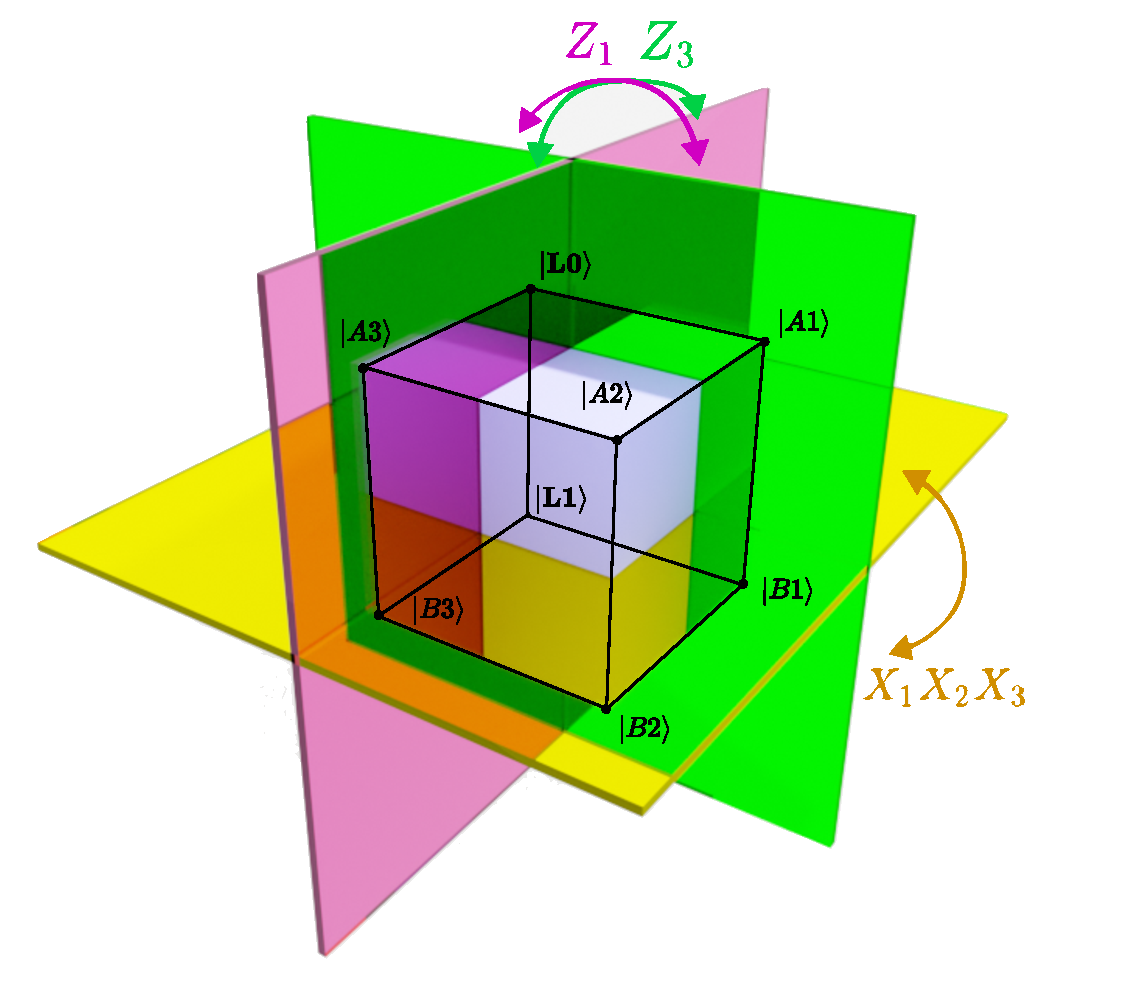
\includegraphics[scale = 0.6]{Figures/group/group.pdf}
    \caption{Group structure of the $n=3$ locked states and error states. Starting from the locked states, phase and bit flip errors with a combination of reflections in the planes shown.
    }\label{fig:group}
\end{figure}
Now suppose a bit-flip or error flip occurs on any of the qubits. Then 
\begin{align*}
    Z_1\ket{L0} = -X_1\ket{L1} = &(\ket{000} - \ket{011} + \ket{101} + \ket{110})/2 = \ket{A1}\\
    X_1\ket{L0} = Z_1\ket{L1} = &(\ket{100} - \ket{111} + \ket{001} + \ket{010})/2 = \ket{B1}
\end{align*} with $\ket{A2},\ket{A3},\ket{B2},\ket{B3}$ defined similary. The three generators of the group $\mathbb{Z}_2\times\mathbb{Z}_2\times\mathbb{Z}_2$ can be mapped to $Z_1, Z_3$ and $X_1X_2X_3$ which defines a representation of this group acting on the 3 qubit Hilbert space. The 8 group elements can be mapped to the identity, the three phase-flips, the three bit-flips, and a phase-and-bit flip that takes $\ket{L0}$ to $\ket{L1}$, an instantaneous process for which there would be no clear mechanism. It is clear, therefore, that any combination of these errors will keep the state within this set of states.

\begin{figure}[h]
    \centering
    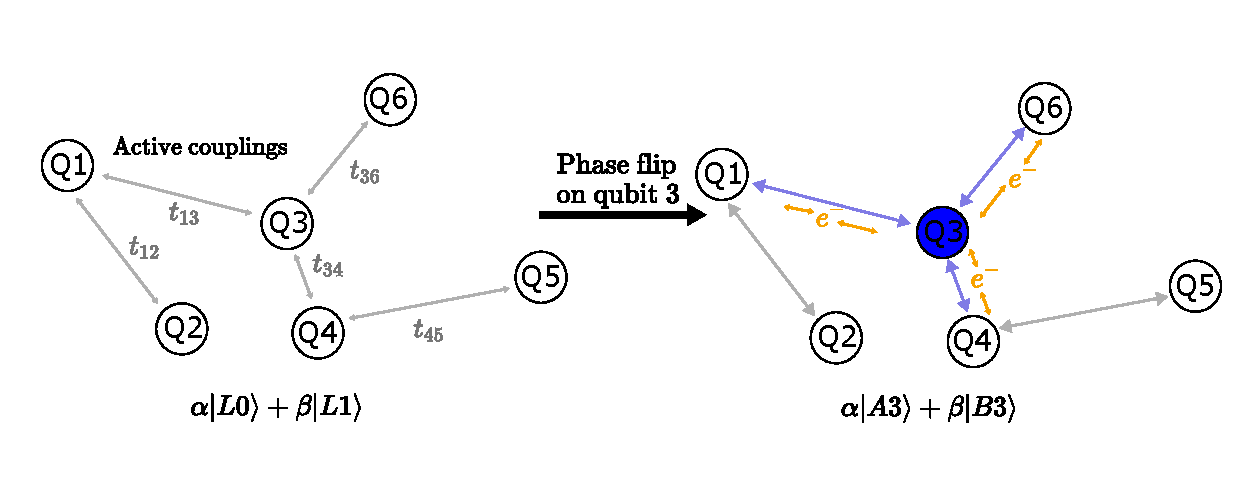
\includegraphics[scale = 0.8]{Figures/locked_states.pdf}
    \caption{The locked property of a locked state. In the codespace, spanned by $\ket{L0}$ and $\ket{L1}$, no electrons can `move' (i.e. the state is uncoupled to the doubly occupied states). If, for example, a phase flip occurs on qubit 3, then the state moves into the $\ket{A3}, \ket{B3}$ error subspace. In this subspace, electrons are free to hop between qubit 3 and the neighbouring qubits where there is a coupling applied. This can perhaps be detected by a charge sensor.
    }\label{fig:lockedstates}
\end{figure}

The states $\ket{Ai}$ and $\ket{Bi}$ have the property that turning on the hopping term in the Hubbard Hamiltonian between qubit $i$ and any other qubit $j$ will now result in a non-zero coupling to the the relevant doubly occupied states. If a potential difference is applied to encourage tunneling, this double occupation will be registered on a charge sensor. The nature of the wavefuntion collapse in this case is somewhat unclear.
\subsubsection{Creating the locked states}
Despite their apparent complexity, these states can be created using a quantum circuit with depth that is linear in the number of qubits. I will give the n-qubit circuit, and illustrate the effects for clarity on the $n = 3$ case.

Start with a single ancilla qubit and the n qubits which we want to turn into a locked state and apply a Hadamard gate to each of this latter group:
\begin{equation*}
    \ket{0}\ket{000}\xrightarrow{H^{\otimes n}} \ket{0}(\ket{000} + \ket{001} + \ket{010} + \ket{011} + \ket{100} + \ket{101} + \ket{110} + \ket{111})/\sqrt{8}
\end{equation*}.
Then apply a $Rz(\pi/2)$ rotation to every qubit:
\begin{equation*}
    \xrightarrow{Rz(\pi/2)^{\otimes n}} \ket{0}(\ket{000} + i\ket{001} + i \ket{010} - \ket{011} + i \ket{100} - \ket{101} - \ket{110} -i \ket{111})/\sqrt{8}
\end{equation*}. Now apply controlled X gates, conditioned on each qubit and targeting the ancilla:
\begin{align*}
    \xrightarrow{\prod_i^\otimes{CX(i,0)}} &\frac{\ket{0}}{4}(\ket{000} - \ket{011} - \ket{101} - \ket{110})
    + \frac{i\ket{1}}{4}(\ket{001} + \ket{010} + \ket{100} - \ket{111})\\
    = &\frac{\ket{0}}{\sqrt(2)}\ket{L0} + \frac{i\ket{1}}{\sqrt(2)}\ket{L1}
\end{align*}. We now need to configure this into a general linear combination of $\ket{L0}$ and $\ket{L1}$.
\begin{align*}
    \xrightarrow{Rz_0(-\pi/2)} &\frac{\ket{0}}{\sqrt(2)}\ket{L0} + \frac{\ket{1}}{\sqrt(2)}\ket{L1}\\
    \xrightarrow{\prod_i^\otimes{CX(0,i)}} & \frac{\ket{0} + \ket{1}}{\sqrt{2}}\ket{L0}\\
    \xrightarrow{U} & (\alpha\ket{0} + \beta\ket{1})\ket{L0}\\
    \xrightarrow{\prod_i^\otimes{CX(i,0)}} & \alpha\ket{0}\ket{L0} + \beta\ket{1}\ket{L1}
\end{align*}
\subsubsection{Error detection and correction}
It is clear from the above how these locked states could be used for an error detection scheme. It is less clear to what extent these states could be used for error correction. An outline scheme could be:
Start with two groups of qubits, each in a locked state, with no $t$ coupling between them, in the codespace:
\begin{equation*}
    \ket{\psi(0)} = \alpha\ket{L0}\ket{L0} + \beta\ket{L1}\ket{L1}
\end{equation*}. Now suppose a phase flip occurs in the second qubit of the second group of qubits:
\begin{align*}
    \xrightarrow{Z_2,2} &\alpha\ket{L0}\ket{A2} + \beta\ket{L1}\ket{B2}\\
    =&\alpha\ket{L0}(-\ket{1\mathbf{01}} + \ket{111} + \ket{1\mathbf{10}}+\ket{011})/2 + \beta\ket{L1}(-\ket{0\mathbf{10}} + \ket{000} + \ket{0\mathbf{01}}+\ket{100})/2.
\end{align*}
This allows electrons to hop between qubits 1 and 2, and between 2 and 3 of the second group. The component of double occupation should cause the system to collapse into a charge eigenstate with double occupation on one of the three qubits. If the system then relaxes back into the computational basis, perhaps due to the potential difference being lowered, the only trace of which type of error ocurred will remain on the unaffected qubit in the second group. In the example above, the charge hops between qubits 2 and 3 of the second group (in bold). The single occupation states must collapse away, and we are left with, after relaxation:
\begin{align*}
    \rightarrow\alpha\ket{L0}\ket{110} + \beta\ket{L1}\ket{010}.
\end{align*}. We can use an ancilla qubit and a series of $CX$ gates with the qubits of the first locked state to find out which error ocurred:
\begin{align*}
    \xrightarrow{\text{ancilla}} & \ket{0}(\alpha\ket{L0}\ket{110} + \beta\ket{L1}\ket{010})
    \xrightarrow{\prod_i^\otimes CX(i,0)}\alpha\ket{0}\ket{L0}\ket{110} + \beta\ket{0}\ket{L1}\ket{010}
\end{align*}. We can then apply the following projective measurement:
\begin{align*}
    P_1 = \ket{00}\bra{00} + \ket{11}\bra{11} && P_2 = \ket{01}\bra{01} + \ket{10}\bra{10}
\end{align*}
where the first and second qubit represent the ancilla qubit and the first qubit of the second group respectively. This tells us the error sydrome, and it is just a matter of applying more $CX$ gates following the construction procedure detailed above to return the system to the codespace.
\end{appendices}
\end{document}